
% np.sqrt()
% np.round( , num_decimals)
% np query syntax
% np.append
% np.flip
% two kinds of sorting
% remove (by index  and by value?)

% indexing, slices

\chapter[Associative arrays in Python (2 of 3)]{\huge\selectfont{Associative
arrays in Python (2 of 3)}}
\label{ch:assocArraysInPython2}

\index{series@\texttt{Series} (Pandas)}
K, now we can create \texttt{Series}es; let's figure out what we can do with
them.

\section{Accessing individual elements}

\index{element}
\index{len@\texttt{len()}}

We can use the same \texttt{len()} function in yet a third way: to ascertain
the number of key/value pairs in a series. Using the Figure~\ref{fig:Series}
example (p.~\pageref{fig:Series}):

\begin{Verbatim}[fontsize=\small,samepage=true,frame=single,framesep=3mm]
print(len(alter_egos))
\end{Verbatim}

\begin{Verbatim}[fontsize=\small,samepage=true,frame=leftline,framesep=5mm,framerule=1mm]
4
\end{Verbatim}

\index{boxies (square brackets)}
\index{[]@\texttt{[]} (boxies)}

Accessing the value for a given key uses exactly the same syntax that NumPy
arrays used (boxies), except with the key in place of the numeric index:

\begin{Verbatim}[fontsize=\small,samepage=true,frame=single,framesep=3mm]
superhero = alter_egos['Peter']
print("Pssst...Peter is really {}.".format(superhero))
\end{Verbatim}

\begin{Verbatim}[fontsize=\small,samepage=true,frame=leftline,framesep=5mm,framerule=1mm]
Pssst...Peter is really Spidey.
\end{Verbatim}

\index{uniqueness!of keys in an associative array}

This is why it's important that the \textit{keys} of an associative array be
unique, even though the \textit{values} often aren't. If we type
``\texttt{alter\_egos[\textquotesingle Peter\textquotesingle]},'' we need to
get back one well-defined answer, not an ambiguous set of
alternatives.\footnote{Pandas, which tries to be All Things To All
People\texttrademark, will actually let you have duplicate index values in a
\texttt{Series}. What does it do if you ask for ``the'' value of
\texttt{Peter}, then, if there's more than one? It gives you back another
\textit{\texttt{Series}} of the different \texttt{Peter} superheroes. This is a
major pain, because now when you look up a value in the \texttt{Series}, you
don't know whether you'll get back a single item or another \texttt{Series},
which means you have to check to see which one it is, and then write different
code to handle the two cases...yick. Just stay far, far away. Make all your
keys unique.}

To overwrite the value for a key with a new value, just treat it as a variable
and go:

\begin{Verbatim}[fontsize=\small,samepage=true,frame=single,framesep=3mm]
alter_egos['Bruce'] = 'Batman'
print(alter_egos)
\end{Verbatim}

\begin{Verbatim}[fontsize=\small,samepage=true,frame=leftline,framesep=5mm,framerule=1mm]
Bruce      Batman
Peter      Spidey
Tony     Iron Man
Thor         Thor
dtype: object
\end{Verbatim}

This same syntax works for adding an entirely \textit{new} key/value pair as
well:

\begin{Verbatim}[fontsize=\small,samepage=true,frame=single,framesep=3mm]
alter_egos['Diana'] = 'Wonder Woman'
print(alter_egos)
\end{Verbatim}

\begin{Verbatim}[fontsize=\small,samepage=true,frame=leftline,framesep=5mm,framerule=1mm]
Bruce          Batman
Peter          Spidey
Tony         Iron Man
Thor             Thor
Diana    Wonder Woman
dtype: object
\end{Verbatim}

It's just like with ordinary variables, if you think about it. Saying
``\texttt{x=5}'' overwrites the current value of \texttt{x} if there already
\textit{is} an \texttt{x}, otherwise it creates a new variable \texttt{x} with
that value.

\index{del operator@\texttt{del} operator (Pandas)}
\label{delOp}

Finally, to outright remove a key/value pair, you use the \texttt{del}
operator:

\begin{Verbatim}[fontsize=\small,samepage=true,frame=single,framesep=3mm]
del alter_egos['Tony']
print(alter_egos)
\end{Verbatim}

\begin{Verbatim}[fontsize=\small,samepage=true,frame=leftline,framesep=5mm,framerule=1mm]
Bruce          Batman
Peter          Spidey
Thor             Thor
Diana    Wonder Woman
dtype: object
\end{Verbatim}

Bye bye, Iron Man.

\index{in place@``in place''}

Don't get mad when I tell you that all of the above operations work
\textbf{in place} on the \texttt{Series}, which is very different than some of
the ``return a modified copy'' style we've seen recently. Hence all of these
attempts are \textit{wrong}:

\begin{Verbatim}[fontsize=\small,samepage=true,frame=single,framesep=3mm]
alter_egos = del alter_egos['Tony']                   <--- WRONG!
alter_egos = alter_egos['Bruce'] = 'Batman'           <--- WRONG!
alter_egos = alter_egos['Diana'] = 'Wonder Woman'     <--- WRONG!
\end{Verbatim}

You don't ``change a value and get a new \texttt{Series}''; you just
``change it.''

\subsection{Accessing by position}

\index{order}

One slightly weird thing you can do with a Pandas \texttt{Series} is ignore the
key (index) altogether and instead use \textit{the number of the key/value
pair} to specify what value you want. This gives me the heebie-jeebies, because
as I explained back on p.~\pageref{assocArraysUnordered}, there really isn't
any meaningful ``order'' to the key/value pairs of an associative array. In
true All Things To All People\texttrademark~fashion, however, Pandas lets you
do this.

\subsubsection{Accessing a value by position}

\label{iloc}
\index{iloc@\texttt{.iloc} syntax (Pandas)}

You can ask for the value of (say) ``the second'' superhero. To do so, you use
the bizarrely-named \textbf{.iloc syntax}:

\begin{Verbatim}[fontsize=\small,samepage=true,frame=single,framesep=3mm]
a_hero = alter_egos.iloc[1]
print(a_hero)
\end{Verbatim}
\vspace{-.3in}

\begin{Verbatim}[fontsize=\small,samepage=true,frame=leftline,framesep=5mm,framerule=1mm]
Spidey
\end{Verbatim}

This is occasionally useful, so I mention it for completeness. The
\texttt{.iloc} numbers start with 0 (not 1) as is true throughout Python.

\subsubsection{Accessing a key by position}

\index{index@\texttt{.index} syntax (Pandas)}
\label{dotIndex}

Similarly, you can get the \textit{key} (as opposed to the value) of the
key/value pair at a particular position. To ask for the key of ``the second''
superhero, you use the \textbf{.index syntax}:

\begin{Verbatim}[fontsize=\small,samepage=true,frame=single,framesep=3mm]
a_secret_hero = alter_egos.index[1]
print(a_secret_hero)
\end{Verbatim}
\vspace{-.3in}

\begin{Verbatim}[fontsize=\small,samepage=true,frame=leftline,framesep=5mm,framerule=1mm]
Peter
\end{Verbatim}


\section{Vectorized arithmetic operators}

As with NumPy \texttt{ndarrays}, you can apply arithmetic operators like
\texttt{+} and \texttt{*} to entire \texttt{Series}es at a time, which is not
only easy code to write but also runs blazing fast. But the Pandas
\texttt{Series} is even smarter than that.

\begin{figure}[ht]
\centering
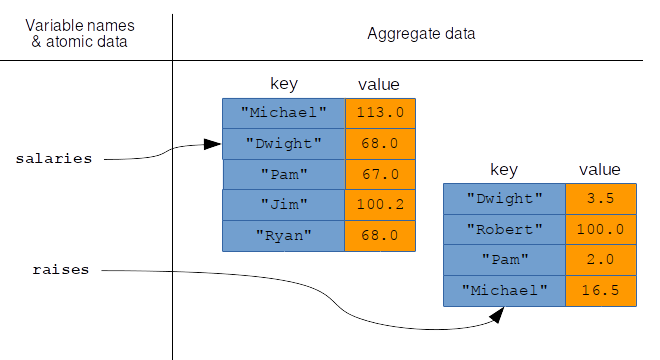
\includegraphics[width=0.9\textwidth]{vectorizedPandas.png}
\caption{Two \texttt{Series}es in memory}
\label{fig:vectorizedPandas}
\end{figure}

Consider the memory picture in Figure~\ref{fig:vectorizedPandas}. Here we have
two \texttt{Series}es, one pointed to by a \texttt{salaries} variable and the
other by \texttt{raises}, which are of different sizes and which have
overlapping, but not identical, sets of keys. What do you suppose Pandas would
do if we executed this code?

\begin{Verbatim}[fontsize=\small,samepage=true,frame=single,framesep=3mm]
new_salaries = salaries + raises
\end{Verbatim}

The answer, happily, is the smartest possible thing it could do. Pandas gets
neither confused nor stifled by the fact that the keys are in different orders
in the two \texttt{Series}es, and instead it does what you surely want:
add corresponding elements, with matching keys, and produce a new
\texttt{Series} with all of those sums.

\begin{figure}[ht]
\centering
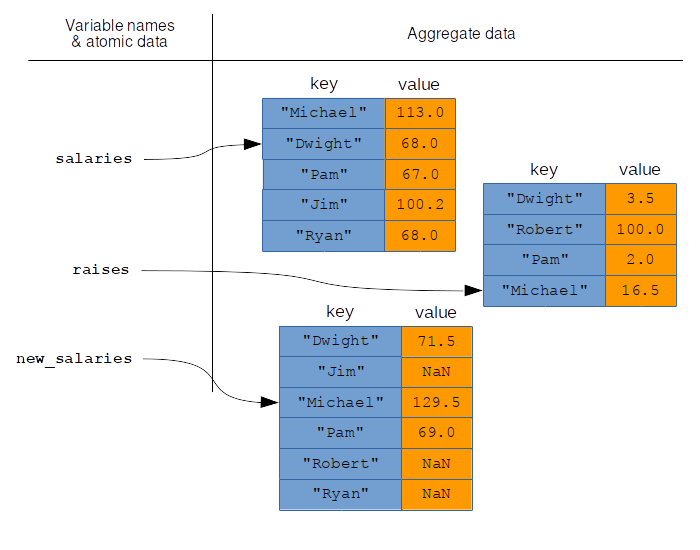
\includegraphics[width=0.8\textwidth]{vectorizedPandas2.png}
\caption{The result of \texttt{+}'ing two \texttt{Series}es that don't have all the same keys.}
\label{fig:vectorizedPandas2}
\end{figure}

The actual result in this case is in Figure~\ref{fig:vectorizedPandas2}, and
the output is here:

% salaries = pd.Series([113,68,67,100.2,68],
%   index=['Michael','Dwight','Pam','Jim','Ryan'])
% raises = pd.Series([3.5,100,2,16.5],
%   index=['Dwight','Robert','Pam','Michael'])

\begin{Verbatim}[fontsize=\small,samepage=true,frame=single,framesep=3mm]
new_salaries = salaries + raises
print(new_salaries)
\end{Verbatim}

\begin{Verbatim}[fontsize=\small,samepage=true,frame=leftline,framesep=5mm,framerule=1mm]
Dwight      71.5
Jim          NaN
Michael    129.5
Pam         69.0
Robert       NaN
Ryan         NaN
dtype: float64
\end{Verbatim}

\index{nan@\texttt{NaN} (``not a number'')}
\index{missing value}

Convince yourself that \texttt{Dwight}'s \$68,000 salary got added to his
\$3,500 raise, and that \texttt{Michael}'s \$113,000 was added to \$16,500,
\textit{etc.}

\label{NaN}

Don't get freaked out by those \texttt{NaN} entries just yet. The special value
``\textbf{NaN}'' stands for ``\textbf{not a number},'' and basically means that
Pandas has to throw up its hands in that case. And with good cause.
\texttt{Jim} has a current salary of \$100,200 in the first \texttt{Series},
but has no value at all in the second one (no raise for Jim this year? Haven't
decided what his raise will be yet? Something else?) and so Pandas shrugs and
says ``dunno.'' We say that the \texttt{Jim} entry in the
\texttt{new\_salaries} \texttt{Series} is a \textbf{missing value}. The same is
true for \texttt{Robert} and \texttt{Ryan}, each of whom was present in only
one of the two operands.

Now I know what you're thinking: ``can't Pandas just assume the salary and/or
raise is 0 if there's a missing one?'' The answer is that yes it can, but it
won't do so unless you give the go-ahead. Pandas is being cautious here, and
doesn't want to introduce errors into your data stream by false assumptions.
(Maybe in your company, for instance, there's a default entry-level salary that
every employee receives who's unspecified in the \texttt{salary}
\texttt{Series}. Or maybe the yearly raise is always assumed to be a flat 2.5\%
cost-of-living raise unless explicitly specified.)

\index{add@\texttt{add()} function (Pandas)}
\index{sub@\texttt{sub()} function (Pandas)}
\index{mul@\texttt{mul()} function (Pandas)}
\index{div@\texttt{div()} function (Pandas)}

If we do want Pandas to assume a certain default value, we have to change
tactics a bit and go with the \texttt{add()} function (or \texttt{sub()},
\texttt{mul()}, or \texttt{div()}):

\begin{Verbatim}[fontsize=\small,samepage=true,frame=single]
new_salaries = pd.Series.add(salaries, raises, fill_value=0)
print(new_salaries)
\end{Verbatim}

\begin{Verbatim}[fontsize=\small,samepage=true,frame=leftline,framesep=5mm,framerule=1mm]
Dwight      71.5
Jim        100.2
Michael    129.5
Pam         69.0
Robert     100.0
Ryan        68.0
dtype: float64
\end{Verbatim}

The \texttt{fill\_value} argument is the important one here: it specifies what
default value to use if one of the addends is missing a key from the other. Now
the result is as in Figure~\ref{fig:vectorizedPandas3}. You can, of course,
choose a \texttt{fill\_value} other than zero, if you wish.

\begin{figure}[ht]
\centering
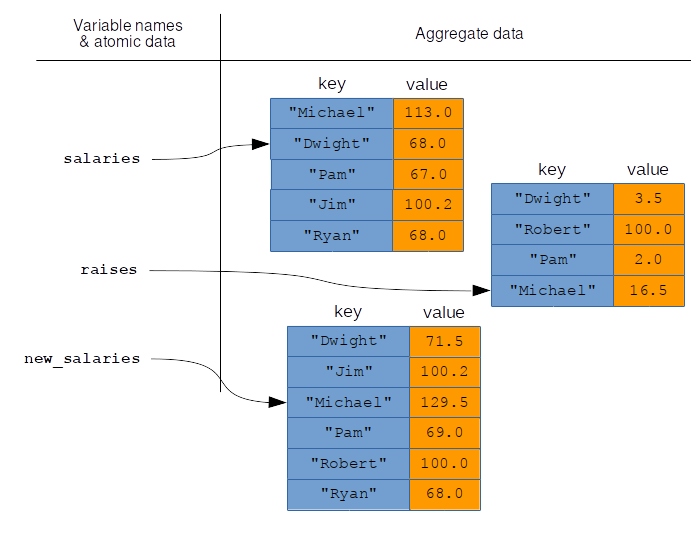
\includegraphics[width=0.8\textwidth]{vectorizedPandas3.png}
\caption{Using \texttt{add()} instead, and passing a \texttt{fill\_value}.}
\label{fig:vectorizedPandas3}
\end{figure}

As with NumPy arrays, we can add (or subtract, or multiply, ...) a single
atomic value to a series as well:

\begin{Verbatim}[fontsize=\small,samepage=true,frame=single,framesep=3mm]
cost_of_living_increase = salaries * .025
print(cost_of_living_increase)
\end{Verbatim}

\begin{Verbatim}[fontsize=\small,samepage=true,frame=leftline,framesep=5mm,framerule=1mm]
Michael    2.825
Dwight     1.700
Pam        1.675
Jim        2.505
Ryan       1.700
dtype: float64
\end{Verbatim}

\begin{Verbatim}[fontsize=\small,samepage=true,frame=single,framesep=3mm]
salaries = salaries + cost_of_living_increase
print(salaries)
\end{Verbatim}

\begin{Verbatim}[fontsize=\small,samepage=true,frame=leftline,framesep=5mm,framerule=1mm]
Michael    115.825
Dwight      69.700
Pam         68.675
Jim        102.705
Ryan        69.700
dtype: float64
\end{Verbatim}

It can sometimes be useful to do string concatenation as well, for instance if
we had employee first names and last names in two \texttt{Series}es with their
employee ID as the index:

\begin{Verbatim}[fontsize=\small,samepage=true,frame=single,framesep=3mm]
firsts = pd.Series(['Hannibal', 'Clarice', 'Multiple', 'Buffalo'],
    index=[666, 1993, 47, 988])
lasts = pd.Series(['Starling', 'Crawford', 'Lecter', 'Bill', 'Miggs'],
    index=[1993, 1650, 666, 988, 47])
print(firsts + " " + lasts)
\end{Verbatim}

\begin{Verbatim}[fontsize=\small,samepage=true,frame=leftline,framesep=5mm,framerule=1mm]
47        Multiple Miggs
666      Hannibal Lecter
988         Buffalo Bill
1650                 NaN
1993    Clarice Starling
dtype: object
\end{Verbatim}

\section{Copying \texttt{Series}es}

\index{copying@copying (\texttt{Series}es)}
The rules for copying (or not copying) \texttt{Series}es are exactly the same
as for NumPy arrays (see Section~\ref{copyingNotCopyingArrays} on
p.~\pageref{copyingNotCopyingArrays}). If you merely assign one \texttt{Series}
object to another variable, the two variables will be pointing to the
\textit{same} \texttt{Series} in memory, which means that changes to one will
be reflected in the other. Calling the \texttt{.copy()} method, however,
creates an entirely new \texttt{Series} in memory.

Make sure you understand the following output to confirm your understanding of
this:

\index{Buffy the Vampire Slayer@\textit{Buffy the Vampire Slayer}}

\begin{Verbatim}[fontsize=\scriptsize,samepage=true,frame=single,framesep=3mm]
slayers = pd.Series([120, 72, 200], index=['Buffy','Xander','Willow'])
anti_vamps = slayers
good_guys = slayers.copy()
anti_vamps['Rubert'] = 150
print(slayers)
\end{Verbatim}
\vspace{-.3in}

\begin{Verbatim}[fontsize=\scriptsize,samepage=true,frame=leftline,framesep=5mm,framerule=1mm]
Buffy     120
Xander     72
Willow    200
Rubert    150
dtype: int64
\end{Verbatim}

\begin{Verbatim}[fontsize=\scriptsize,samepage=true,frame=single,framesep=3mm]
print(anti_vamps)
\end{Verbatim}
\vspace{-.3in}

\begin{Verbatim}[fontsize=\scriptsize,samepage=true,frame=leftline,framesep=5mm,framerule=1mm]
Buffy     120
Xander     72
Willow    200
Rubert    150
dtype: int64
\end{Verbatim}

\begin{Verbatim}[fontsize=\scriptsize,samepage=true,frame=single,framesep=3mm]
print(good_guys)
\end{Verbatim}
\vspace{-.3in}

\begin{Verbatim}[fontsize=\scriptsize,samepage=true,frame=leftline,framesep=5mm,framerule=1mm]
Buffy     120
Xander     72
Willow    200
dtype: int64
\end{Verbatim}

(The numbers here are approximate IQs; don't mean to be a hater.)


\section{Sorting \texttt{Series}es}
\index{sorting@sorting (\texttt{Series}es)}
\index{sort\_values@\texttt{.sort\_values()} method (Pandas)}
\index{sort\_index@\texttt{.sort\_index()} method (Pandas)}

Sorting is slightly more complex than for arrays, since there are two things we
might want to sort by: the \texttt{Series}' index, or the values themselves.
Correspondingly, there are two methods: \texttt{.sort\_index()} and
\texttt{.sort\_values()}:

\begin{Verbatim}[fontsize=\small,samepage=true,frame=single,framesep=3mm]
print(anti_vamps.sort_index())
\end{Verbatim}
\vspace{-.3in}

\begin{Verbatim}[fontsize=\small,samepage=true,frame=leftline,framesep=5mm,framerule=1mm]
Buffy     120
Rubert    150
Willow    200
Xander     72
dtype: int64
\end{Verbatim}

\begin{Verbatim}[fontsize=\small,samepage=true,frame=single,framesep=3mm]
print(anti_vamps.sort_values())
\end{Verbatim}
\vspace{-.3in}

\begin{Verbatim}[fontsize=\small,samepage=true,frame=leftline,framesep=5mm,framerule=1mm]
Xander     72
Buffy     120
Rubert    150
Willow    200
dtype: int64
\end{Verbatim}

\index{in place@``in place''}
Like NumPy's \texttt{np.sort()} function (but unlike its \texttt{.sort()}
method; refer back to Section~\ref{sortingArrays} on p.~\pageref{sortingArrays}
for details), neither of these methods actually sort the \texttt{Series} in
place; instead, they return sorted copies. However, they can be made to, by
including ``\texttt{inplace=True}'' as an argument:

\begin{Verbatim}[fontsize=\small,samepage=true,frame=single,framesep=3mm]
heroes_dumb_to_smart = anti_vamps.sort_values()
print(heroes_dumb_to_smart)
\end{Verbatim}
\vspace{-.3in}

\begin{Verbatim}[fontsize=\small,samepage=true,frame=leftline,framesep=5mm,framerule=1mm]
Xander     72
Buffy     120
Rubert    150
Willow    200
dtype: int64
\end{Verbatim}

\begin{Verbatim}[fontsize=\small,samepage=true,frame=single,framesep=3mm]
print(anti_vamps)
\end{Verbatim}
\vspace{-.3in}

\begin{Verbatim}[fontsize=\small,samepage=true,frame=leftline,framesep=5mm,framerule=1mm]
Buffy     120
Xander     72
Willow    200
Rubert    150
dtype: int64
\end{Verbatim}

\begin{Verbatim}[fontsize=\small,samepage=true,frame=single,framesep=3mm]
anti_vamps.sort_values(inplace=True)
print(anti_vamps)
\end{Verbatim}
\vspace{-.3in}

\begin{Verbatim}[fontsize=\small,samepage=true,frame=leftline,framesep=5mm,framerule=1mm]
Xander     72
Buffy     120
Rubert    150
Willow    200
dtype: int64
\end{Verbatim}

Another useful feature of both \texttt{.sort\_X} methods is the ability to
\textit{reverse} sort. By adding ``\texttt{ascending=False}'' as an argument
(with or without also including the ``\texttt{inplace=True}'' argument; they
are combinable with a comma) you produce the reverse order:

\begin{Verbatim}[fontsize=\small,samepage=true,frame=single,framesep=3mm]
heroes_smart_to_dumb = anti_vamps.sort_values(ascending=False)
print(heroes_smart_to_dumb)
\end{Verbatim}
\vspace{-.3in}

\begin{Verbatim}[fontsize=\small,samepage=true,frame=leftline,framesep=5mm,framerule=1mm]
Willow    200
Rubert    150
Buffy     120
Xander     72
dtype: int64
\end{Verbatim}

\begin{Verbatim}[fontsize=\small,samepage=true,frame=single,framesep=3mm]
anti_vamps.sort_index(inplace=True, ascending=False)
print(anti_vamps)
\end{Verbatim}
\vspace{-.3in}

\begin{Verbatim}[fontsize=\small,samepage=true,frame=leftline,framesep=5mm,framerule=1mm]
Xander     72
Willow    200
Rubert    150
Buffy     120
dtype: int64
\end{Verbatim}

\section{Concatenating and combining}

\index{uniqueness!of keys in an associative array}
Finally, it is sometimes convenient to be able to combine two or more
\texttt{Series}es into a single one. But there's a catch. Remember that in
order for a \texttt{Series} to ``work properly,'' its keys must be unique.
Combining two \texttt{Series} which share at least one of the same keys is a
recipe for disaster!

The syntax for doing so, when the coast is clear, uses the \texttt{.append()}
method:

\begin{Verbatim}[fontsize=\small,samepage=true,frame=single,framesep=3mm]
crazy_example = salaries.append(slayers)
print(crazy_example)
\end{Verbatim}
\vspace{-.3in}

\begin{Verbatim}[fontsize=\small,samepage=true,frame=leftline,framesep=5mm,framerule=1mm]
Michael    113.0
Dwight      68.0
Pam         67.0
Jim        100.2
Ryan        68.0
Xander      72.0
Willow     200.0
Rubert     150.0
Buffy      120.0
dtype: float64
\end{Verbatim}

Nothing untoward happened here because \textit{The Office} and \textit{Buffy}
don't have any overlapping character names. Note that the values all got
converted to \texttt{float} (instead of \texttt{int}), to enforce homogeneity.
Note also that \texttt{salaries} itself did \textit{not} change as a result of
this \texttt{.append()} call; instead, a new \texttt{Series} was returned that
contains all the items.


\section{Summary}

All the functions from this chapter are summarized in
Figure~\ref{fig:handySeries}.

\setlength\extrarowheight{5pt}

\begin{figure}[ht]
\centering
\begin{tabular}{c|p{3.3in}}
Function & Description \\
\hline

\texttt{len(}\textsl{ser}\texttt{)} & Get the number of key/value pairs in the
\texttt{Series} \textsl{ser}. \\

\textsl{ser}\texttt{[\textquotesingle Five Guys\textquotesingle]} & Get the value of a specific key from the
\texttt{Series} \textsl{ser}. \\

\textsl{ser}\texttt{.iloc[73]} & Treating the key/values pairs in the
\texttt{Series} \textsl{ser} as ordered, get a specific numbered (from 0)
value. \\

\textsl{ser}\texttt{.index[73]} & Treating the key/values pairs in the
\texttt{Series} \textsl{ser} as ordered, get a specific numbered (from 0)
key. \\

\textsl{ser}\texttt{[\textquotesingle Firehouse\textquotesingle] =} (\textsl{something}) & Set the value for a key of
the \texttt{Series} \textsl{ser}. \\

\textsl{ser}\texttt{[\textquotesingle New Rest\textquotesingle] =}
(\textsl{something}) & Add an additional key/value pair to the \texttt{Series}
\textsl{ser}. (Same syntax as the previous.) \\

\textsl{ser} \texttt{+ 13} & Add a quantity to each value of \textsl{ser},
yielding a new \textit{Series}. (Also works with \texttt{-}, \texttt{*},
\texttt{/}, \textit{etc.}) \\

\index{nan@\texttt{NaN} (``not a number'')} \textsl{ser1} \texttt{+}
\textsl{ser2} & Add pairs of values that have matching keys in two
\texttt{Series}es, yielding a new \texttt{Series}. Use \texttt{NaN} for the
value of any key that doesn't appear in both \textsl{ser1} and \textsl{ser2}.
(Also works with \texttt{-}, \texttt{*}, \texttt{/}, \textit{etc.}) \\

\shortstack{\texttt{pd.Series.add(}\textsl{ser1}\texttt{,}\\\quad\quad\quad\textsl{ser2}\texttt{,
fill\_value=}\textsl{x})} & Add pairs of values that have matching keys in two
\texttt{Series}es, yielding a new \texttt{Series}. Use \texttt{x} for any
missing values. (Also works with \texttt{sub()}, \texttt{mul()},
\texttt{div()}, \textit{etc.}) \\

\textsl{ser1} = \textsl{ser2} & Make \textsl{ser1} point to the same data that
\textsl{ser2} points to. (\textit{Not} a copy!)\\

\textsl{ser1} = \textsl{ser2}\texttt{.copy()} & Make \textsl{ser1} point to a
new, independent copy of \textsl{ser2}. \\

\textsl{ser}\texttt{.sort\_index()} & Return a copy of the \texttt{Series}
\textsl{ser} which is sorted by the keys. Can also pass
``\texttt{inplace=True}'' to change \textsl{ser} itself, and/or pass
``\texttt{ascending=False}'' to get reverse order. \\

\textsl{ser}\texttt{.sort\_values()} & Same as above, except that sorting is
done with respect to values, not keys. \\

\textsl{ser1}\texttt{.append(}\textsl{ser2}\texttt{)} & 
Return a new \texttt{Series} with \textsl{ser1}'s and \textsl{ser2}'s key/value
pairs smooshed together. (Bad things may happen if \textsl{ser1} and
\textsl{ser2} share some of the same keys.) \\

\end{tabular}
\bigskip
\caption{Handy functions, methods, and operators for Pandas \texttt{Series}es.}
\label{fig:handySeries}
\end{figure}
